\documentclass[11pt]{report}
% \usepackage[utf8]{inputenc} % pictures
\usepackage[titletoc]{appendix} % appendix
\usepackage{nopageno} % Disable bottom page #
\usepackage{multicol} % multicolumn 
\usepackage{enumitem} % list items
\usepackage{fancyhdr} % page headers
\usepackage{titlesec} % title format

% Graphics library for displaying pictures
\usepackage{graphicx}
\graphicspath{ {images/} }

\usepackage{tabu} % allows for tables with width control

% Setting the margins
\usepackage[top=.5in, left=1in, bottom=1in, right=1in]{geometry}
 
% bibliography stuff, to compile use
% user@host~$ pdflatex file.tex
% user@host~$ bibtex file.tex 
% user@host~$ pdflatex file.tex
%
\usepackage[backend=bibtex]{biblatex}
\addbibresource{final_report.bib}

% Create clickable table of contents
\usepackage{hyperref}
\hypersetup {colorlinks,
    citecolor=black,
    filecolor=black,
    linkcolor=black,
    urlcolor=black
}

% Fix itemize spacing
\newenvironment{myitemize}
{ \begin{itemize}
    \setlength{\itemsep}{0pt}
    \setlength{\parskip}{0pt}
    \setlength{\parsep}{0pt}     }
{ \end{itemize}                  } 

%set font style
\renewcommand\familydefault{\sfdefault}

% Set line spacing
\renewcommand{\baselinestretch}{1}

% Set indent size
\setlength\parindent{0pt}

% column spacing
\setlength\columnsep{4pt}

% Title format
\titleformat{\chapter}{\Huge\bf}{\thechapter}{20px}{\Huge\bf}


\begin{document}
% Begining of title page

{\Huge \textbf{CS 320 Course Project Final Report:}}
\vspace{5mm}
\begin{flushright}

    {\huge for}
    \vspace{20mm}

    \textbf{\Huge Vaultron}
    \vspace{20mm}

    {\huge Version $<0.0.1>$}
    \vspace{20mm}

    {\huge Prepared by}
    \vspace{20mm}

    \textbf{\huge Cryptomaniacs}
    \vspace{20mm}
\end{flushright}

\begin{multicols}{3}
    \noindent
    \begin{itemize}
        \item[] {\Large Colton King}
        \item[] {\Large Grant Wade}
        \item[] {\Large Robby Boney}
        \item[] {\Large Rob Wooner}
    \end{itemize}

    \begin{itemize}
        \item[] {\Large 11245746}
        \item[] {\Large 11435949}
        \item[] {\Large 11453444}
        \item[] {\Large 11496643}
    \end{itemize}

    \begin{itemize}
        \item[] {\Large\texttt colton.king@wsu.edu}
        \item[] {\Large\texttt grant.wade@wsu.edu}
        \item[] {\Large\texttt robby.boney@wsu.edu}
        \item[] {\Large\texttt robert.wooner@wsu.edu}
    \end{itemize}
\end{multicols}

\vfill

\begin{flushright}
    \vspace{20mm}
    {\Large \textbf{Date:} Sunday, December 10th, 2017}
\end{flushright}

% Begining of second page
\clearpage


\tableofcontents{}

\chapter{Introduction}

\section{Project Overview}
Vaultron is a cryptographically secure cross platform password manager
written in electron and node.js which allows users to store their account
information for websites locally with easy access.


\section{Definitions, Acronyms And Abbreviations}
\textbf{CSS:} Cascading Style Sheets, used to style our electron application

\textbf{Electron:} Cross platform desktop application development environment
using HTML, CSS, and JavaScript

\textbf{node.js:} JavaScript runtime built on Chrome's V8 JavaScript engine. Used
for file io and backend applications.

\textbf{HTML:} HyperText Markup Language, used to design our electron application

\textbf{JavaScript:} Programming language used on the web and Electron

\textbf{Vault:} Password storage platform created for this project

\textbf{PBKDF2:} Password Based Key Derivation Function v2


\section{References And Acknowledgments}

    \nocite{*}
    \printbibliography[heading=none]



% END OF INTRODUCTION

\chapter{Design}

\section{System Modeling}
At the 



\section{Interface Design}
Following are visualizations the windows for our application and brief 
descriptions of their purpose to the app.

\subsection{Login}
This window is where the user starts from and allows them to create an account
or login into a previously existing one with their masterpassword.

\begin{center}
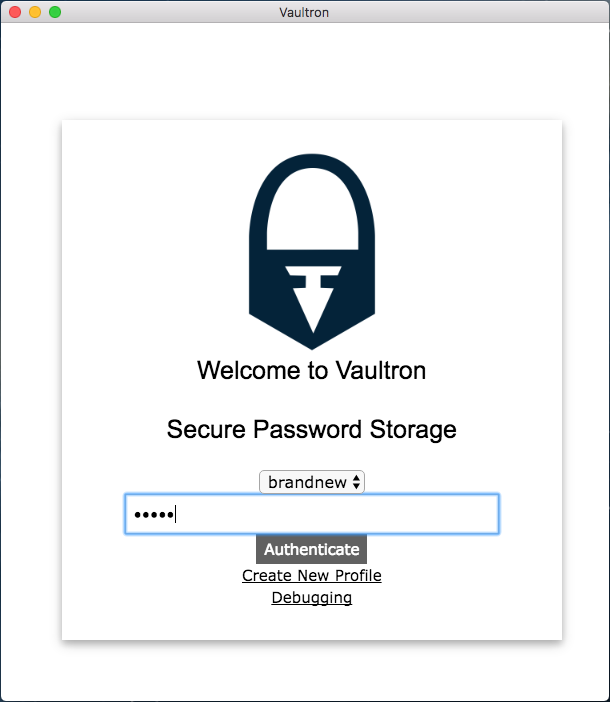
\includegraphics[scale=0.50]{app-login-demo.png}
\end{center}

\subsection{Main App}
The main window that displays the vault content and allows the user to navigate
to other aspects of the app such as password generation or entry creation.

\begin{center}
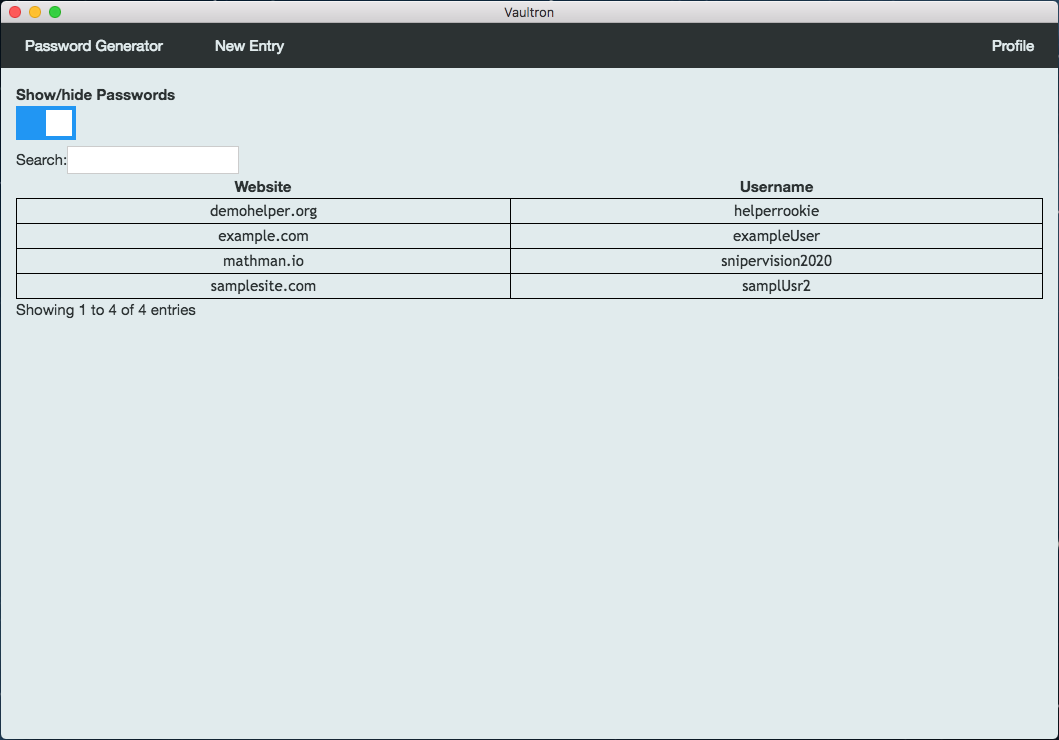
\includegraphics[scale=0.40]{app-main-demo.png}
\end{center}

\subsection{Create Entry}
This window is used to add information to be stored in the vault.
\begin{center}
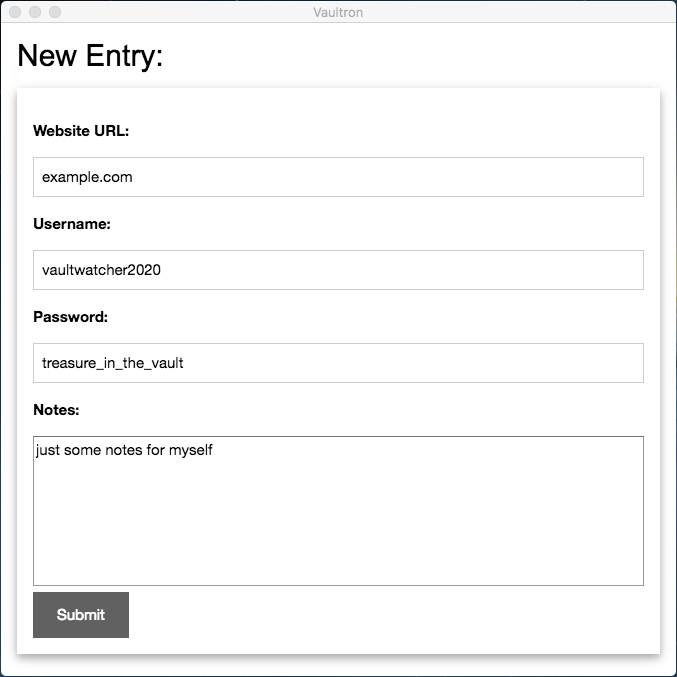
\includegraphics[scale=0.40]{app-newentry-demo.png}
\end{center}

\subsection{Generate Password}
Our tool for users to generate cryptographically secure passwords which can be
used in place of user designed passwords.
\begin{center}
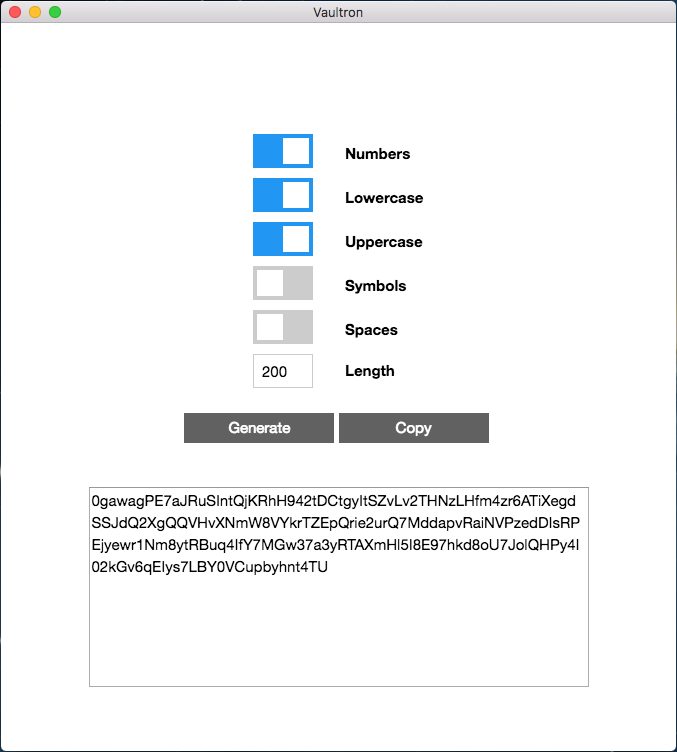
\includegraphics[scale=0.40]{app-passgen-demo.png}
\end{center}

% END OF DESIGN

\chapter{Implementation}

\section{Development Environment}
stuff

\section{Task Distribution}
stuff

\section{Challenges}
Our Journey and its many adventures.


% END OF IMPLEMENTATION


\chapter{Testing}

\section{Testing Plan}
testing


\section{Tests For Functional Requirements}
testing


\section{Tests For Non-Functional Requirements}
Testing

\section{Hardware And Software Requirements}
Testing

% END OF TESTING


\chapter{Analysis}
stuff about analysis

% END OF Analysis


\chapter{Conclusion}
stuff about analysis

% END OF CONCLUSION


\begin{appendices}

    \chapter{Group Log}
    \begin{itemize}
        \item Meeting 1: Sunday, October 8th: Discussed project ideas and began writing SRS. 3 hours
        \item Meeting 2: Monday, October 9th: Finished first two chapters of SRS. 1 hour
        \item Meeting 3: Wednesday, October 11th: Wrote majority of chapters 3 and 4. 2 hours
        \item Remote Work: 10-12 hours via Discord/Github
        \item Colton: Wrote sections 1.2, 2.6, 3.1.1, 3.1.2, 4.1, Data dictionary
        \item Grant: Designed SRS, and wrote sections 1.3, 2.7, 3.1.4, 4.2, 4.3
        \item Rob: Designed SRS, and wrote sections 2.3, 2.5, 3.1.3, 3.2, 3.3
        \item Robby: Designed diagrams, references, and wrote sections 1.5, 1.6, 2.1, 2.4, 3.3.1
    \end{itemize}


\end{appendices}

\end{document}
